%%
%%%%%%%%%%%%%%%%%%%%%%% file typeinst.tex %%%%%%%%%%%%%%%%%%%%%%%%%
%
% This is the LaTeX source for the instructions to authors using
% the LaTeX document class 'llncs.cls' for contributions to
% the Lecture Notes in Computer Sciences series.
% http://www.springer.com/lncs       Springer Heidelberg 2006/05/04
%%
% It may be used as a template for your own input - copy it
% to a new file with a new name and use it as the basis
% for your article.
%
% NB: the document class 'llncs' has its own and detailed documentation, see
% ftp://ftp.springer.de/data/pubftp/pub/tex/latex/llncs/latex2e/llncsdoc.pdf
%
%%%%%%%%%%%%%%%%%%%%%%%%%%%%%%%%%%%%%%%%%%%%%%%%%%%%%%%%%%%%%%%%%%%


\documentclass[runningheads,a4paper]{llncs}

\usepackage{amssymb}
\usepackage{apacite}
\usepackage{caption}
\usepackage{feynmp}
\usepackage{multirow}
\usepackage{bm}
\usepackage{siunitx}
\usepackage{xfrac}
\usepackage{enumitem}
\DeclareGraphicsRule{*}{mps}{*}{}
\usepackage[compat=1.1.0]{tikz-feynman}

\setcounter{tocdepth}{3}
\usepackage{graphicx}
\usepackage{cancel}
\usepackage[intlimits]{amsmath} % Puts the limits of integrals on top and bottom
\usepackage{amsxtra}     % Use various AMS packages
%\usepackage{amsthm}
\usepackage{amssymb}
\usepackage{amsfonts}
\usepackage{graphicx}    % Add some packages for figures. Read epslatex.pdf on ctan.tug.org
\usepackage{rotating}
\usepackage{color}
\usepackage{epsfig}
%\usepackage{subcaption}   % To make subfigures. Read subfigure.pdf on ctan.tug.org
\usepackage{float}

\newcommand{\sun}{\ensuremath{\odot}} % sun symbol is \sun
\newcommand{\metrel}{$E_{\text T}^{\text {miss,rel}}$}
\newcommand{\dileptonmass}{$m_{\ell \ell}$}
\newcommand{\mttwo}{$m_{\text{T2}}$}
\newcommand{\invfb}{fb\textsuperscript{-1}}
\newcommand{\lumi}{$\int \mathcal{L} \, \mathrm{dt}$}
\newcommand{\met}{$E_{\text T}^{\text {miss}}$}

\usepackage{url}
\urldef{\mailsa}\path|{a.garayjalloh, d.gowdastorz, |
\urldef{\mailsb}\path|m.fingerhuth, s.natarajan, h.rice, |
\urldef{\mailsc}\path|annabel.wolf}@student.maastrichtuniversity.nl|    
\newcommand{\keywords}[1]{\par\addvspace\baselineskip
\noindent\keywordname\enspace\ignorespaces#1}

\begin{document}

\mainmatter  % start of an individual contribution

% first the title is needed
\title{-- DRAFT VERSION --\\LHC Data Challenge\\Establishing a Bound on the Higgs Boson Mass}

% a short form should be given in case it is too long for the running head
\titlerunning{Establishing a Bound on the Higgs Boson Mass}

% the name(s) of the author(s) follow(s) next
%
% NB: Chinese authors should write their first names(s) in front of
% their surnames. This ensures that the names appear correctly in
% the running heads and the author index.
%
\author{Adam Garay Jalloh%
%\thanks{Please note that the LNCS Editorial assumes that all authors have used
%the western naming convention, with given names preceding surnames. This determines
%the structure of the names in the running heads and the author index.}%
\and Dhruva Gowda Storz\and Mark Fingerhuth\and Samuel Natarajan\and\ Henry Rice\and Annabel Wolf}
%
\authorrunning{LHC Data Challenge}
% (feature abused for this document to repeat the title also on left hand pages)

% the affiliations are given next; don't give your e-mail address
% unless you accept that it will be published
\institute{Maastricht Science Programme, Maastricht University,\\
Maastricht, The Netherlands\\
\mailsa\\
\mailsb\\
\mailsc\\
}

%
% NB: a more complex sample for affiliations and the mapping to the
% corresponding authors can be found in the file "llncs.dem"
% (search for the string "\mainmatter" where a contribution starts).
% "llncs.dem" accompanies the document class "llncs.cls".
%

\toctitle{Lecture Notes in Computer Science}
\tocauthor{Authors' Instructions}
\maketitle


\begin{abstract}
The abstract should summarize the contents of the paper and should
contain at least 70 and at most 150 words. It should be written using the
\emph{abstract} environment.
\keywords{We would like to encourage you to list your keywords within
the abstract section}
\end{abstract}

%%SAM & AN START

\section{Introduction}

The Large Hadron Collider, located in CERN, Geneva, is the largest and most powerful particle accelerator in the world. It consists of a ring, about 27 kilometres in circumference, with a number of accelerating structures to increase the energy of the particles along the way. Within the loop there are two channels surrounded by superconducting magnets which allow the charged particles to be accelerated in opposite directions. The LHC is used by an international team of scientists to investigate the nature of the universe. The main objectives are to understand the shortcomings of the standard model; to explain the origin of mass using the Higgs field, to discover the reason for the missing anti-matter of the universe, and to understand the nature of dark matter and dark energy. Furthermore, supersymmetry is investigated, because this might unify the four fundamental forces by including gravity in the Standard Model.

This report discusses data collected from the ATLAS detector in 2012, which was released publicly in June 2016. It will give an overview of the most important background processes and explain how a signal is distinguished from the background. Furthermore, the statistical analysis of potential new physics is discussed.

\subsection{The LHC and ATLAS}

ATLAS, A Toroidal LHC Apparatus, is one of the four main particle detectors located along the LHC, where proton collision experiments are conducted. Two high-energy particle beams, each with 2808 bunches of ${10}_{11}$ protons, travel through the accelerator close to the speed of light in an ultrahigh vacuum (${10}_{–13}$ atm) and at a temperature of $-271.3$°C in opposite direction. The two beams are aligned to collide inside the ATLAS detector, which uses a large array of detectors organised in cylindrical shells to measure the properties of the particles passing through them. 

Each layer of the detector reconstructs different particles. The first layer consists of tracking devices, which show the tracks of electrically charged particles through the trails they leave by ionizing matter. The particle’s momentum can be determined by measuring the curvature of the trajectory. Tracking devices either consist of a gaseous chamber or a semiconductor detector. In gaseous chambers, electrons or ions are collected on electrodes under a strong electric field, whereas semiconductor detectors are based on the fact that electron-hole pairs are created when particles pass through a reverse-biased semiconductor. The next layer of the detector is an electromagnetic calorimeter. This absorbs all electrons and photons, which have electromagnetic properties. Hadrons begin to lose energy in this stage, but are not stopped until they reach the hadronic calorimeter. The final layer of the detector catches muons. See Fig. \ref{fig:atlas} for a schematic overview. \cite{aad2012observation}

\begin{figure}
\centering
\includegraphics[height=7cm]{atlas}
\caption{Overview of the different layer of the ATLAS detector. Retrieved from:
http://atlas-opendata.web.cern.ch/atlas-opendata/webanalysis/}
\label{fig:atlas}
\end{figure}

\subsection{The Standard Model}

The Standard Model is a rigorously tested mathematical model that describes the properties and interactions of elementary particles. It is a quantum field theory, relating The standard model is composed of three generations of quarks and leptons, four gauge bosons and the Higgs boson (see Fig. \ref{fig:standardmodel}). The formulation of The mathematical formula used to make calculations for the standard model is known as the Lagrangian equation. The Standard Model has resulted in the prediction and subsequent discovery of the Higgs Boson; the mode of interaction between energy and space-time, resulting in particles with mass.

\begin{figure}
\centering
\includegraphics[height=6.5cm]{standardmodel}
\caption{The fermions and bosons described by the Standard Model}
\label{fig:standardmodel}
\end{figure}

Every elementary particle can be said to have a corresponding field residing within space-time. The motion of particles can be described by ripples in their respective fields. Each of these fields is considered to be a quantum mechanical operator that has the ability to create particles out of the ground-state or vacuum (therefore, is able to violate the law of conservation of mass and momentum). The creation of particles is comparable to ripples in the field that move through space-time. \cite{raby1997neutrino} There are four fundamental quantum fields for mass particles (quarks and leptons), electroweak bosons, gluons, and the Higgs boson.

The up and down quarks make up the first generation of particles and are the lightest and most stable. All stable matter in the universe consists of first generation particles. Second (c and s) and third (t and b) generations are less stable and heavier. Quarks come in different colours and only mix in such ways as to form colourless objects.

Leptons are also arranged in three generations (1st column 1st generation, etc.). The electron, muon and tau are electrically charged and have mass, but the neutrinos are neutral and have very little mass.

Weak, electromagnetic and strong forces result from the exchange of force-carrier particles, which are all bosons. The strong force is carried by the gluon, electromagnetic force by photon and weak force by W and Z bosons.

The Higgs boson is one of the most recent discoveries in the field of particle physics and It has been postulated that its interaction with the Higgs field creates a “friction” on the particle. This friction limits the particle’s energy so that it can no longer travel at the speed of light, and consequently creates mass. \cite{melnikov2010w+}

\textbf{Mathematics behind the measurements}


Protons are composed of quarks and gluons which are released in "jets" at the point of collision. The particles of interest, which scientists intend to study, are usually present directly after the collisions. These particles then decay into other particles (usually more stable ones with lighter mass) with the mediation of force carriers, or Bosons. This process can be best described with a feynman diagram.

Importantly, charge and momentum are conserved during the decay process, allowing us to extract the invariant mass of the original particle. The decay process can happen several times before anything is measured in the detector. Furthermore, several decay processes can produce the same stable particles. Considering these factors, it can be difficult to isolate the target decay process when there are millions of events happening in each proton bunch. In this sense there is a considerable quantity of background "noise" which must be filtered out of the data to correctly identify processes of interest.

\textbf{Background signals}

When scientists first developed the standard model, many of the predicted elementary particles had not yet been observed or studied. When these particles slowly began to be understood and tested against the standard model, the questions surrounding them dissipated as well and became factual interpretation of large sums of data. Once predictions have been validated sufficiently, the particles are accepted as part of the standard model and become so-called "background processes". In other words, the particles which are well established and understood are no longer the target of measurements.

What physically differentiates the signal from the background is that the signal must be equal to, or in excess of five sigma difference between itself and the background. This enforces a scientific standard for uncertainty in measurements and prevents improperly validated speculation.

When searching for particular signals (for example, two bosons decaying into four leptons) one must consider that many other decay process produce the same stable particles. In order to differentiate the ZZ signal from these background events, ATLAS strategically looks at data in regions which produce the same leptons, and then extrapolates that to the signal region. 

%% SAM & AN END


%% DHRUVA START
As the Large Hadron Collider accellerates particles close to the speed of light, it leaves the territory of classical mechanics and enters that of relativity. This manifests mathematically and provides new tools to calculate and predict important features of a collision. One of the most elementary changes brought about by this change is the use of 4-vectors instead of 3-vectors \cite{griffithsintroduction}. 3-vectors as used in classical mechanics only have three components which represent the x, the y and the z axes. 4 vectors on the other hand, while still representing the same thing as its counterpart 3-vector, make use of time as their 0th component. The time component is multiplied by the speed of light to give it the same units as the other components. 
4 vectors are useful as the momentum 4 vector makes it relatively straightforward to do momentum calculations in collisions. The momentum 4-vector has energy as its 0th component, which proves extremely useful due to Einstein’s famous equation 

\begin{equation}
{ E }^{ 2 }\quad ={ \quad (pc) }^{ 2 }\quad +\quad { (m{ c }^{ 2 }) }^{ 2 }
\end{equation}

Using this, we can see that at relativistic speeds, the momentum, mass and energy are closely related. Using this relationship and energy/momentum conservation laws, one can reconstruct collision events from the fragments encountered by the detectors more easily.

In order to reconstruct events, we first and foremost need data. What data we need depends on the situation we are looking at. The most common data made use of at CERN is the invariant mass, the missing transverse energy, and the reconstructed mass. 

The Invariant Mass or relativistic mass needs to be introduced as mass changes as a particle accelerates. The invariant mass is the mass of a body at rest \cite{helliwell2010special}. The mass at a certain velocity can then be calculated by transforming the rest mass by a factor of gamma. In a decay, invariant mass is conserved, so it can be used to reconstruct the mass of the decaying particle. It is assumed in most cases that the total mass of the fragments of a decay is equal to the mass of the decaying particle. Off-shell particles and relativistic masses provide exceptions to this, but a histogram of the total invariant mass often results in a bell curve with a peak at the mass of the decaying particle. 

Sometimes, one encounters a case where the momenta of the fragments dont add up to that of the colliding particles. This manifests itself as missing transverse energy. This phenomenon is due to the production of particles that cannot be detected by the detectors. A prime example is the neutrino, which is capable of passing through large bodies of matter without interacting with it. Neutrino production is observed quite often in several phenomenon such as in W decays. By calculating exactly how much energy is missing in the collision, one can use the missing energy as a value for the invariant mass of the produced neutrino and carry out calculations to recreate the original decay from this information. Since the actual mass of the neutrino is not known, we can calculate a reconstructed mass for the decaying particle (the W boson in this case). This mass is known as the reconstructed mass or mτ. As an example to illustrate this, the formula \cite{http://physics.stackexchange.com_13ADAD} to calculate the reconstructed transverse mass of a W boson is as follows 

\begin{equation}
{ m }_{ T }\quad =\quad \sqrt { 2{ p }_{ T }^{ l }{ p }_{ T }^{ v }(1-cos\Delta { \phi  }_{ lv }) }
\end{equation}
 
where ${ p }_{ T }^{ l }$ represents the momentum of the lepton, ${ p }_{ T }^{ v }$ represents the momentum of the neutrino (which is assumed to be the missing energy), and $\Delta { \phi  }_{ lv }$ represents the angle between the lepton and the neutrino’s trajectory. 

%% DHRUVA END

%% SAM START

\section{Computational Methods}

Particle physics is highly dependent on competent programming and software engineering to make sense of the quantum world that scientists seek to explore. Programming is a vastly adaptable and versatile tool that enables data collection, storage, management, modelling, analysis, plotting and fitting.

This project utilized Ubuntu, which is a Linux operating system, for managing the large sums of data from ATLAS in a more hands-on, customizable environment. It was necessary to install an OS with a C++ compiler in order to run a piece of code that processed all the events in a number of selected datasets. This processed data could then be graphed in Histograms allowing for further analytical processing. The programming environment ‘terminal’ was used, which is a command-line window that compiles C++. C++ is a useful language in this scenario as it allows for classes to inherit properties from their base class. For example, the class Z Boson extends the base class Boson and therefore inherits an integer only spin.

In most cases the events that occur in the LHC are very unpredictable processes and often only part of the entire process is recorded by the particle detectors. For this reason, Monte-Carlo simulation methods are used to model and infer the outcomes of the full range of processes. These simulate the conditions and parameters that are conducive for new-physics processes and shows scientists what to expect when the actual data is collected.

%% SAM END

%% HENRY START

\subsection{Statistics}

New events are observed continuously, but in order to identify whether these new effects are significant or not to the Standard Model a key requirement is to propose a null hypothesis, stating that there are no fluctuations in the data set, and an alternative hypothesis, that there has been a fluctuations in the data set. In the interest of finding new particles the null hypothesis must be rejected, hence the event selected will be found in the tail of the distribution. In other words significance is the probability that by mistake one rejects the null hypothesis. Typically a 5σ value is used to assess the confidence level, p-value, of the data collection. In high energy physics (HED) the selection of a steep confidence level is done to distinguish whether it is a measurement (5 σ), an observation (a p-value of 4σ is needed) or if there is evidence (a p-value of 3σ is needed) for the event taking place if more time were invested in the researched of this physical effect. (http://www.hep.caltech.edu/~fcp/statistics/lectures0802/L0802B.pdf)

To perform more meaningful significance estimates a blind analysis approach is usually always conducted, in essence designing the analysis before a glimpse is even taken into the results. The reason is to handle the data in this manner is to already know the specific cuts to make so reducing the possibility of the wanted or another interesting signal which in the future might be an interesting background.  The cuts are picked following the extensive data provided by MonteCarlo simulations, the already known background processes and furthermore QED behaviors involved with the physical variable under consideration which may have led to a systematic error.
 
The level of significance, how well the cuts were carried out, is given by the score function. The score function is defined as “the sum of the background events, B, and the score function, S, will be equal to the total number of events, N. Hence:

\begin{equation}
S = N - B
\end{equation}

Therefore the uncertainty of S will be the following:

[....]

%% HENRY END

%% MARK START
\section{Background Processes/Signals}

\subsection{Z Decay}

Being the heavy analog of the photon, the neutral Z boson has a mass of $m_{Z}\cong91.2 GeV$ and a cross-section of $\Gamma_{Z}\cong2.5 GeV$. It decays either hadronically or leptonically with a very short half life of $\tau = 1/\Gamma\cong{ 10 }^{ -25 }sec$. This analysis will focus on the leptonic decay mode into two oppositely charged leptons of same flavour as shown in the Feynman diagram in Fig. \ref{fig:feynmzll}.

\begin{figure}
\centering
\includegraphics[height=2.5cm]{feynm_Z}
\caption{Feynman diagram for ${Z}^{0}$ decay}
\label{fig:feynmzll}
\end{figure}

For the single Z analysis the following search criteria were employed:
\begin{itemize}
\item Two good leptons with ${p}_{T} > 25$ GeV
\item Leptons must have opposite charge
\item Leptons were required to have same flavour
\end{itemize}
\bigbreak
\textbf{$Z \quad \rightarrow \quad { e }^{ - } \quad + \quad { e }^{ + }$}

The Zee process is one of the main background processes when trying to extract events with two electrons in their final state since it has a relatively high cross section. In order to filter specifically for Zee processes the two good leptons were required to be of lepton type 11, which stands for electrons. The results of running this search on the Zee Monte-Carlo simulation are shown below. Fig. \ref{fig:invmzee} plots the frequency distribution against mass (GeV) and a distinct peak at $\sim$90 GeV can be seen, which is a good estimate for the Z mass.

\begin{figure}
\centering
\includegraphics[height=3.7cm]{InvM_Zee_fit}
\caption{Invariant mass histogram for Zee decay}
\label{fig:invmzee}
\end{figure}

The analysis of background processes also requires the familiarization with plots of different parameter spaces such as plotting the frequency distribution against missing transverse energy. This plot, visualized in Fig. \ref{fig:mtezee}, exhibits a linear decrease in MET until 200 GeV and then contains a peak centered around roughly 250 GeV.

\begin{figure}
\centering
\includegraphics[height=3.7cm]{MTE_Zee+new}
\caption{Missing transverse energy histogram for Zee process}
\label{fig:mtezee}
\end{figure}

Furthermore, the number of jets was plotted against frequency and is demonstrated in Fig. \ref{fig:nojzee}. It can be concluded, that small jets have a much higher prevalence for Zee processes than large number of jets. All in all, the conducted Z analysis revealed distinct patterns in the frequency plots of MET, invariant mass and number of jets that can be exploited in subsequent searches by introducing cutoff values for the parameters.

\begin{figure}
\centering
\includegraphics[height=3.7cm]{NoJ_Zee+new}
\caption{Histogram for the number of jets for the Zee process}
\label{fig:nojzee}
\end{figure}
\bigbreak
$Z\quad \rightarrow \quad { \mu  }^{ - }\quad +\quad { \mu  }^{ + }$
\smallbreak
Since the Z boson can decay into any two leptons of the same flavour, the decay into two muons ($\mu$), each with a mass of 105.7 MeV, also needs to be considered. Compared to the previous search, only the lepton type was changed to 13, signifying muons instead of electrons. The search was conducted on the Zmumu MC data set and the invariant mass was again plotted against the frequency distribution and the resulting histogram is shown in Fig. \ref{fig:invmzmumu}. The Gaussian fit clearly shows a peak centered around $\sim$90 GeV which constitutes another good approximation of the Z mass. It should be noted that Fig. \ref{fig:invmzee} and \ref{fig:invmzmumu} look very similar, implying that the two processes have roughly the same cross section. [can I say that?]

\begin{figure}
\centering
\includegraphics[height=3.7cm]{InvM_Zmumu_fit}
\caption{Invariant mass histogram for Zmumu decay}
\label{fig:invmzmumu}
\end{figure}

Fig. \ref{fig:mtezmumu} shows the MTE histogram, which demonstrates that there is much less MTE in Zmumu processes compared to Zee processes. After a small peak at 30 GeV the MTE frequency rapidly approaches zero and all MTE is found below 100 GeV. Since there are no neutrinos involved in the Zmumu decay process, no MTE is expected and, hence, the entire MET in Zee and Zmumu processes is considered “fake” MTE. This special type of MTE is attributed to wrong measurements and errors such as incorrectly classifying jet energy as MTE. A distinct feature of “fake” MTE is its fast convergence to zero and the resulting small tails in the MTE histogram as seen in Fig. \ref{fig:mtezmumu}.

\begin{figure}
\centering
\includegraphics[height=3.7cm]{MTE_Zmumu_new}
\caption{Missing transverse energy histogram for Zmumu process}
\label{fig:mtezmumu}
\end{figure}

When incorrectly measured jet energy is indeed the cause of the MTE distribution obtained in Fig. \ref{fig:mtezmumu}, it expected that the MTE vector will mostly point in the  direction of the most energetic jet. Therefore, when calculating the difference in azimuthal angle between the MTE vector and the most energetic jet, by definition given by the ${0}^{th}$ entry in the jet\_phi vector, a decreasing frequency distribution is expected with increasing radians. This prediction is verified by the histogram shown in Fig. \ref{fig:deltaphizmumu}. Oscillations are visible in the frequency distribution but no distinct linear increase with radians can be observed. To verify these result the azimuthal angular differences between the second most energetic jets and the MTE vectors were computed and are demonstrated in Fig. 7. Again no increase with radians is observed which implies that the “fake” MTE shown in Fig. \ref{fig:mtezmumu} is probably due to other reasons than incorrectly measured jet energy.

\begin{figure}
\centering
\includegraphics[height=4cm]{deltaphi_jet0_met_Zmumu_fit}
\caption{Distribution of angular difference in azimuthal angle plotted against radians}
\label{fig:deltaphizmumu}
\end{figure}
\bigbreak
$Z\quad \rightarrow \quad \tau ^{ - }\quad +\quad { \tau  }^{ + }$

Besides decaying into electrons and muons, the Z boson can also decay into two tau leptons. However, since tau leptons are very heavy compared to electrons and muons, their cross section and contribution to the background will be relatively low. Furthermore, searching for tau leptons requires much more sophisticated reconstruction methods and it is therefore much more difficult than searching electrons and muons in the final states. Due to all these reasons this decay mode was not searched and analysed further in this paper.

%% MARK END
%% ANN START
\subsection{ZZ Decay}

The decay of two Z bosons is one of the main background processes when searching for the Higgs boson. The decay of ZZ into four good leptons with pT > 10 GeV will be looked at with the following search criteria:

[search criteria] 

[Feynman diagram]

The two Z candidates were required to be built from lepton pairs of opposite charge and same flavour. This minimizes the total deviation of the Z candidates from the mass of the Z boson. The maximal total deviation for the ZZ analysis is set to 20 GeV:

\begin{equation}
|mass Z candidate 1 - mass Z| + |mass Z candidate 2 - mass Z| < 20 GeV.
\end{equation}

Since the mass of a single Z is equal to $\sim$90.2 GeV (reference), the invariant mass of ZZ is always greater than $\sim$180 GeV. This is confirmed in Fig. \ref{fig:invmzz}. As it can be seen from the landau fit, the frequency is greatest at $\sim$220 GeV and drops after this point.

\begin{figure}
\centering
\includegraphics[height=4cm]{MyInvariantMassHistoWtihFit_ZZ}
\caption{Invariant mass histogram for the ZZ decay}
\label{fig:invmzz}
\end{figure}

The number of jets were also plotted, and resulted in a very low number which can be neglected (see Fig. \ref{fig:nojzz}). This result makes sense, because no neutrinos are produced in the ZZ to 4 leptons process.

\begin{figure}
\centering
\includegraphics[height=4cm]{MTEWithFit_ZZ}
\caption{Missing transverse energy for the ZZ process}
\label{fig:mtezz}
\end{figure}

\begin{figure}
\centering
\includegraphics[height=4cm]{NumberOfJets_ZZ}
\caption{Histogram for the number of jets for the ZZ decay}
\label{fig:nojzz}
\end{figure}
%%ANN END

%%MARK START
\subsection{W Analysis}

The spin-1 ${W}^{+}$ and ${W}^{-}$ are the only charged bosons in the Standard Model and together with the neutral Z boson they mediate the weak interaction. W bosons have a mass of $m_{W}\cong 80.4 GeV$ and a cross-section of $\Gamma_{Z}\cong2.1 GeV$. With a branching fraction of $\sim67\%$ the W boson mostly decays hadronically, however, this analysis will only focus on the leptonic decay with $\sim11\%$ branching fraction for each lepton generation \cite{Agashe:2014kda}. Depending on its charge the W boson decays into either a positive lepton and a neutrino or a negative lepton and an anti-neutrino as depicted in the Feynman diagrams below (Fig. \ref{fig:feynmw+} and \ref{fig:feynmw-}). Similar to the Z, the W bosons have a very short half life of $\tau = 1/\Gamma\cong{ 10 }^{ -25 }sec$.

\begin{figure}
\centering
\includegraphics[height=2.5cm]{feynm_W-}
\caption{Feynman diagram for ${W}^{-}$ decay}
\label{fig:feynmw-}
\end{figure}

\begin{figure}
\centering
\includegraphics[height=2.5cm]{feynm_W+}
\caption{Feynman diagram for ${W}^{+}$ decay}
\label{fig:feynmw+}
\end{figure}

Contrarily to the Z analysis, no invariant mass histograms can be obtained from the W analysis since only one lepton can be detected and measured in the final state whilst the neutrino escapes the detectors without measurement. Hence, the only way to approximate the momentum of the neutrino is to attribute all the $\cancel{\it{E}}_{T}$ to the neutrino and based on this assumption the ${m}_{t}(W)$ can be calculated.

For the single W analysis the following search criteria were employed:
\begin{itemize}
\item Exactly one good lepton with ${p}_{T} > 25$ GeV
\item $\cancel{\it{E}}_{T} > 30$ GeV 
\item ${m}_{t}(W) > 30$ GeV
\end{itemize}

The obtained histogram of ${m}_{t}$ is shown in Fig. \ref{fig:mtw} and the gaussian fit shows a clear peak close to the W mass given in the literature. Fig. \ref{fig:mtwall} shows the W analysis results that was obtained from all events and visualizes the accuracy of the MC simulation when overlayed with the actual data from the E$\gamma$-channel. Furthermore, it demonstrates that single top decay is often misinterpreted as the decay of a W boson.

\begin{figure}
\centering
\includegraphics[height=4cm]{W_rtm_fit}
\caption{Histogram of ${m}_{t}$ for the W decay}
\label{fig:mtw}
\end{figure}

\begin{figure}
\centering
\includegraphics[height=7cm]{ee_rtmw_with_dataegamma}
\caption{Distribution of ${m}_{t}$ over all events}
\label{fig:mtwall}
\end{figure}

The $\cancel{\it{E}}_{T}$ histogram is shown in Fig. \ref{fig:mtewall} and allows for the same conclusions regarding the single top decay and the accuracy of the MC simulations as Fig. \ref{fig:mtwall}. In contrast to the Z decay, the $\cancel{\it{E}}_{T}$ is considered 'real' since the undetectable neutrino in the final state carries energy.

\begin{figure}
\centering
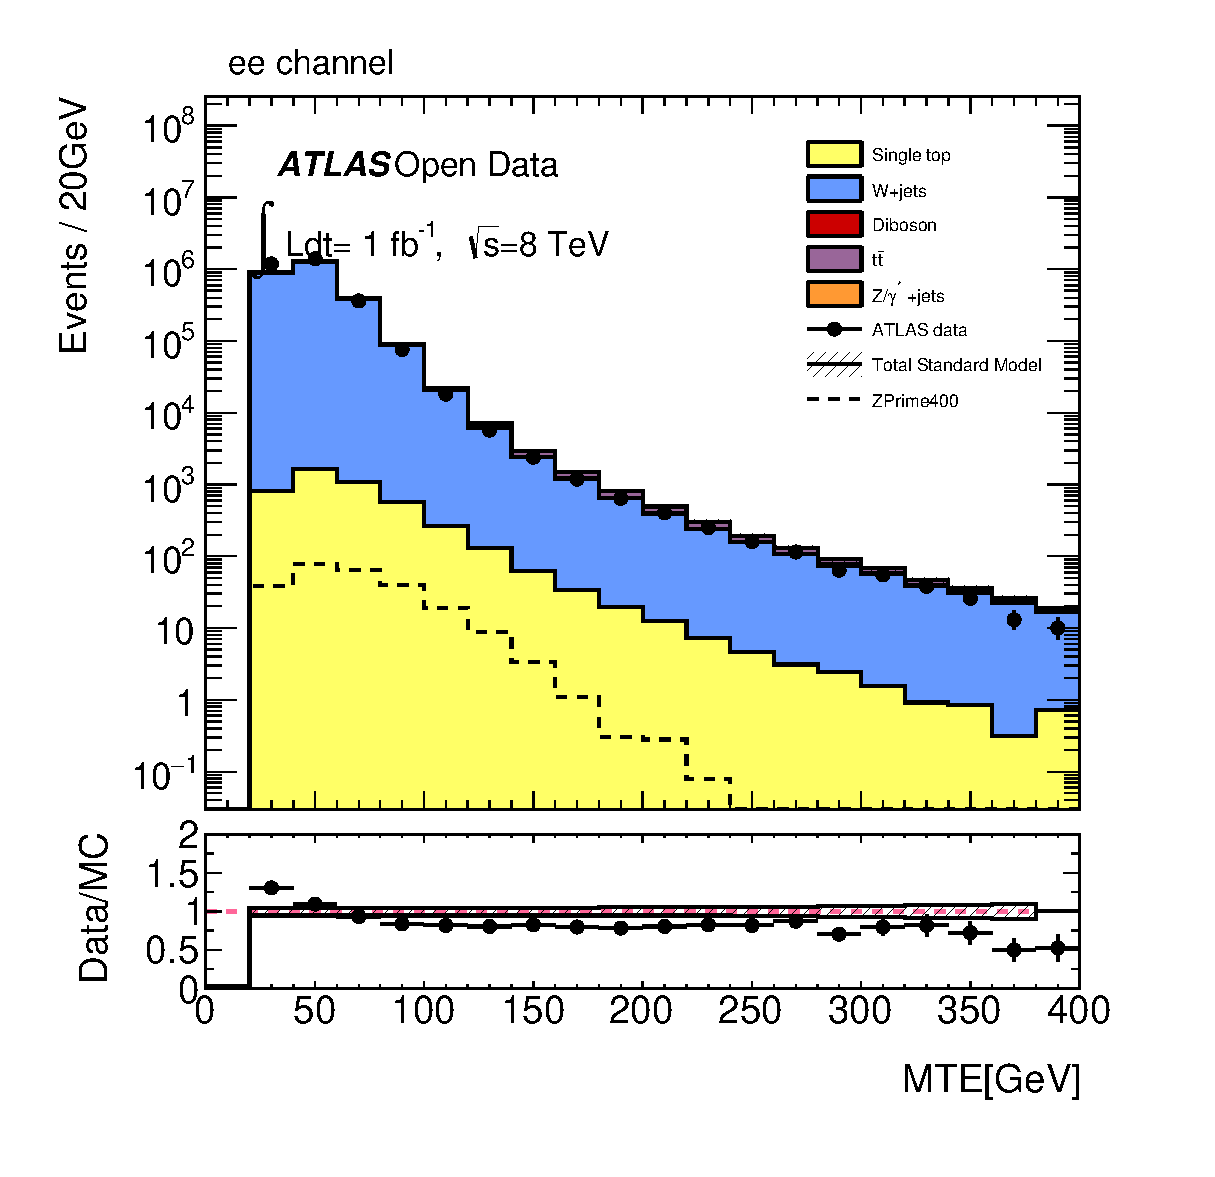
\includegraphics[height=4cm]{ee_mtew_with_dataegamma}
\caption{Missing transverse energy for the W process}
\label{fig:mtewall}
\end{figure}

%% MARK END

%% MARK START
\subsection{Z' search}

The Z' is a new heavy vector boson predicted by many theories that are trying to extend the current SM such as the Sequential Standard Model (SSM) or the ${E}_{6}$ Grand Unified Theory (GUT) model. Based on these models the Z' is expected to have the same couplings as the lighter ${Z}^{0}$ but with a much larger mass in the TeV region. The discovery of a new heavy vector boson is very likely to be one of the first signals for new physics at higher centre-of-mass energies at the LHC. This is due to the fact, that vector bosons generally have high branching fractions for clean decay modes such as leptonic decays and additionally tend to have higher cross-sections than other SM processes. \cite{hayden2013z}\linebreak
\linebreak
Fig. \ref{fig:feynmzprime} shows the Z' decay diagrams which is considered for this search: first decay into a $t$$\overline t$ pair that further decays into a $b$$\overline b$ pair and two W bosons. Subsequently the W bosons decay as well - one hadronically and one leptonically.

\begin{figure}
\centering
\includegraphics[height=5cm]{feynm_ZPrime}
\caption{Feynman diagram for Z' decay}
\label{fig:feynmzprime}
\end{figure}

For this paper the Z' was searched in the semileptonic top pair channel based on the following search criteria:
\begin{itemize}
\item Exactly one good lepton with ${p}_{T} > 25$ GeV
\item Minimum 4 good jets of which two have to be b-tagged
\item $\cancel{\it{E}}_{T} > 30$ GeV 
\item ${m}_{t}(W) + \cancel{\it{E}}_{T} > 30$ GeV
\end{itemize}

\begin{table}[h]
\centering
\captionsetup{width=0.8\textwidth}
\begin{tabular}{|l|llllll}
\hline
Signal models     & \multicolumn{1}{l|}{400-200} & \multicolumn{1}{l|}{600-100} & \multicolumn{1}{l|}{400-200} & \multicolumn{1}{l|}{600-100} & \multicolumn{1}{l|}{400-200} & \multicolumn{1}{l|}{600-100} \\ \hline
\hspace{5mm} \lumi     & \multicolumn{2}{c|}{3.2 \invfb}                                                     & \multicolumn{2}{c|}{9.6 \invfb}                                                     & \multicolumn{2}{c|}{19.2 \invfb}                                                    \\ \hline 
 \mttwo \, cut [GeV]            & \multicolumn{6}{c|}{\textbf{SF channel}}                                                                                                                                                                                                                   \\ \hline
$>80$  & \multicolumn{1}{l|}{1.01}               & \multicolumn{1}{l|}{0.26}               & \multicolumn{1}{l|}{1.74}               & \multicolumn{1}{l|}{0.45}               & \multicolumn{1}{l|}{2.46}               & \multicolumn{1}{l|}{0.64}               \\ \hline
$>100$ & \multicolumn{1}{l|}{1.47}               & \multicolumn{1}{l|}{0.50}               & \multicolumn{1}{l|}{2.56}               & \multicolumn{1}{l|}{0.86}               & \multicolumn{1}{l|}{3.62}               & \multicolumn{1}{l|}{1.22}               \\ \hline
$>120$  & \multicolumn{1}{l|}{1.27}               & \multicolumn{1}{l|}{0.61}               & \multicolumn{1}{l|}{2.19}               & \multicolumn{1}{l|}{1.06}               & \multicolumn{1}{l|}{3.09}               & \multicolumn{1}{l|}{1.5}                \\ \hline
                  & \multicolumn{6}{c|}{\textbf{DF channel}}                                                                                                                                                                                                                  \\ \hline
$>80$   & \multicolumn{1}{l|}{1.12}               & \multicolumn{1}{l|}{0.31}               & \multicolumn{1}{l|}{1.95}               & \multicolumn{1}{l|}{0.54}               & \multicolumn{1}{l|}{2.76}               & \multicolumn{1}{l|}{0.76}               \\ \hline
$>100$   & \multicolumn{1}{l|}{2.10}               & \multicolumn{1}{l|}{0.75}               & \multicolumn{1}{l|}{3.64}               & \multicolumn{1}{l|}{1.30}               & \multicolumn{1}{l|}{5.15}               & \multicolumn{1}{l|}{1.83}               \\ \hline
$>120$    & \multicolumn{1}{l|}{2.10}               & \multicolumn{1}{l|}{1.07}               & \multicolumn{1}{l|}{3.65}               & \multicolumn{1}{l|}{1.86}               & \multicolumn{1}{l|}{5.16}               & \multicolumn{1}{l|}{2.63}               \\ \hline
\end{tabular}
\caption{Significance values ($S/\sqrt{B}$) for the SF and DF channel signal models with various cuts on \mttwo \, at increasing integrated luminosities. Cuts include $Z$ veto (only for SF) and no jets are allowed.}
\label{tab:SF_score}
\end{table}




%% MARK END

%\subsection{Formulas}
%
%Displayed equations or formulas are centered and set on a separate
%line (with an extra line or halfline space above and below). Displayed
%expressions should be numbered for reference. The numbers should be
%consecutive within each section or within the contribution,
%with numbers enclosed in parentheses and set on the right margin --
%which is the default if you use the \emph{equation} environment, e.g.,
%\begin{equation}
%  \psi (u) = \int_{o}^{T} \left[\frac{1}{2}
%  \left(\Lambda_{o}^{-1} u,u\right) + N^{\ast} (-u)\right] dt \;  .
%\end{equation}
%
%Equations should be punctuated in the same way as ordinary
%text but with a small space before the end punctuation mark.
%
%\subsection{Footnotes}
%
%The superscript numeral used to refer to a footnote appears in the text
%either directly after the word to be discussed or -- in relation to a
%phrase or a sentence -- following the punctuation sign (comma,
%semicolon, or period). Footnotes should appear at the bottom of
%the
%normal text area, with a line of about 2~cm set
%immediately above them.\footnote{The footnote numeral is set flush left
%and the text follows with the usual word spacing.}
%
%\subsection{Program Code}
%
%Program listings or program commands in the text are normally set in
%typewriter font, e.g., CMTT10 or Courier.
%
%\medskip
%
%\noindent
%{\it Example of a Computer Program}
%\begin{verbatim}
%program Inflation (Output)
%  {Assuming annual inflation rates of 7%, 8%, and 10%,...
%   years};
%   const
%     MaxYears = 10;
%   var
%     Year: 0..MaxYears;
%     Factor1, Factor2, Factor3: Real;
%   begin
%     Year := 0;
%     Factor1 := 1.0; Factor2 := 1.0; Factor3 := 1.0;
%     WriteLn('Year  7% 8% 10%'); WriteLn;
%     repeat
%       Year := Year + 1;
%       Factor1 := Factor1 * 1.07;
%       Factor2 := Factor2 * 1.08;
%       Factor3 := Factor3 * 1.10;
%       WriteLn(Year:5,Factor1:7:3,Factor2:7:3,Factor3:7:3)
%     until Year = MaxYears
%end.
%\end{verbatim}
%%
%\noindent
%{\small (Example from Jensen K., Wirth N. (1991) Pascal user manual and
%report. Springer, New York)}
%
%\subsection{Citations}
%
%For citations in the text please use
%square brackets and consecutive numbers: -- provided automatically
%by  mechanism.
%
%\subsection{Page Numbering and Running Heads}
%
%There is no need to include page numbers. If your paper title is too
%long to serve as a running head, it will be shortened. Your suggestion
%as to how to shorten it would be most welcome.
%
%\section{LNCS Online}
%
%The online version of the volume will be available in LNCS Online.
%Members of institutes subscribing to the Lecture Notes in Computer
%Science series have access to all the pdfs of all the online
%publications. Non-subscribers can only read as far as the abstracts. If
%they try to go beyond this point, they are automatically asked, whether
%they would like to order the pdf, and are given instructions as to how
%to do so.
%
%Please note that, if your email address is given in your paper,
%it will also be included in the meta data of the online version.
%
%\section{BibTeX Entries}
%
%The correct BibTeX entries for the Lecture Notes in Computer Science
%volumes can be found at the following Website shortly after the
%publication of the book:
%\url{http://www.informatik.uni-trier.de/~ley/db/journals/lncs.html}
%
%\subsubsection*{Acknowledgments.} The heading should be treated as a
%subsubsection heading and should not be assigned a number.
%
%\section{The References Section}\label{references}
%
%In order to permit cross referencing within LNCS-Online, and eventually
%between different publishers and their online databases, LNCS will,
%from now on, be standardizing the format of the references. This new
%feature will increase the visibility of publications and facilitate
%academic research considerably. Please base your references on the
%examples below. References that don't adhere to this style will be
%reformatted by Springer. You should therefore check your references
%thoroughly when you receive the final pdf of your paper.
%The reference section must be complete. You may not omit references.
%Instructions as to where to find a fuller version of the references are
%not permissible.
%
%We only accept references written using the latin alphabet. If the title
%of the book you are referring to is in Russian or Chinese, then please write
%(in Russian) or (in Chinese) at the end of the transcript or translation
%of the title.
%
%The following section shows a sample reference list with entries for
%journal articles 
%Please note that proceedings published in LNCS are not cited with their
%full titles, but with their acronyms!
%
%
%\section*{Appendix: Springer-Author Discount}
%
%LNCS authors are entitled to a 33.3\% discount off all Springer
%publications. Before placing an order, the author should send an email, 
%giving full details of his or her Springer publication,
%to \url{orders-HD-individuals@springer.com} to obtain a so-called token. This token is a \cite{pisani2008periodic}
%number, which must be entered when placing an order via the Internet, in
%order to obtain the discount.
%
%\section{Checklist of Items to be Sent to Volume Editors}
%Here is a checklist of everything the volume editor requires from you:
%
%
%\begin{itemize}
%\settowidth{\leftmargin}{{\Large$\square$}}\advance\leftmargin\labelsep
%\itemsep8pt\relax
%\renewcommand\labelitemi{{\lower1.5pt\hbox{\Large$\square$}}}
%
%\item The final \LaTeX{} source files
%\item A final PDF file
%\item A copyright form, signed by one author on behalf of all of the
%authors of the paper.
%\item A readme giving the name and email address of the
%corresponding author.
%\end{itemize}

\bibliographystyle{apacite}
\bibliography{bookchapter}

\end{document}
